\section{System/Akzeptanztests}
\label{sec:system}

Nun wollen wir am Beispiel einer Suche nach Stellenanzeigen die Entwicklung von Akzeptanztest\index{Test!Akzeptanztest}s und damit die Akzeptanztestgetriebene Softwareentwicklung (vgl. Abschnitt \ref{sec:attd} betrachten.

Zum Einsatz kommt dabei die für Systemtests entwickelte domainspezifische Sprache Cucumber\index{Cucumber} in Verbindung mit der Browser-Steuerung Capybara\index{Capybara}, die beide bereits in Abschnitt \ref{sec:cucumber} vorgestellt wurde. 

Ein Cucumber\index{Cucumber}-Verzeichnis ist qua Konvention immer gleich aufgebaut. In Abbildung \ref{fig:cucumberDir} ist der Verzeichnisbaum, wie er in den Beispielen dieses Kapitels benutzt wird, zu sehen. Innerhalb unseres Projektverzeichnisses existiert ein Unterverzeichnis "`features"' in dem alle Feature-Dateien mit der Endung "`.feature"' lagern. Ebenfalls existiert ein Unterverzeichnis "`step\_definitions"', das die Implementation der Testschritt\index{Cucumber!Testschritt}e beinhaltet, sowie ein Verzeichnis "`support"', für z.B. Standardmethoden, Aktionen die vor jedem Feature-Durchlauf ausgeführt werden, oder die Definition der Browser-Engine. Cucumber lädt automatisch alle Ruby-Dateien in den beiden Verzeichnissen.

\begin{figure}[hbtp]
 \centering
 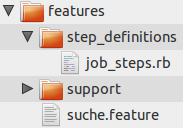
\includegraphics[width=4cm]{./material/cucumber-aufbau.png}
 % cucumber-aufbau.png: 183x128 pixel, 72dpi, 6.46x4.51 cm, bb=
 \caption{Aufbau eines Cucumber- Verzeichnisses}
 \label{fig:cucumberDir}
\end{figure}



\paragraph{1. Definition des gesamten Akzeptanztest\index{Test!Akzeptanztest}}

Zusammen mit dem Kunden, oder basierend auf den Anforderungen entwickeln wir zuerst eine Spezifikation für ein Feature, und darauf aufbauend, Da die Akzeptanztest\index{Test!Akzeptanztest}s in erster Linie dazu dienen, die Software gegenüber den Anfordungen des Kunden zu validieren, und auch als Kommunikationsmittel genutzt wird, orientert sich das Vokabular an gebräuchlichen Begriffen. So ist ein einzelner Testfall ein "`Szenario"' und eine Test-Suite ein "`Feature"'. Statt "`Assertions"' (Zusicherungen) gibt es Vor- und Nachbedingungen.

Nachfolgend sei ein erstes Szenario für eine Suche nach Stellenanzeigen gezeigt.

% Datei: features/suche.feature
% SNIPPET: 
% # language: de                                                                                                                             
% Funktionalität: Job-Suche                                                                                                                  
%   Um Jobs zu finden                                                                                                                        
%   Als ein Gast                                                                                                                             
%   Soll es möglich sein mittels einer Suche Jobs zu finden                                                                                  
%   Szenario: Auffinden durch Titel                                                                                                          
%     Angenommen wir befinden uns auf der Startseite                                                                                         
%     Und die folgenden Jobs sind vorhanden:                                                                                                 
%        | title                    |  visible  |                                                                                            
%        | Ruby on Rails Entwickler |   true    |                                                                                            
%        | Java Programmierer       |   true    |                                                                                            
%     Wenn wir "Rails" für "search" eintippen                                                                                                
%     Und wir auf den Button "Suchen" klicken                                                                                                
%     Dann sehen wir "Ruby on Rails Entwickler"                                                                                              
%                                                                                                                                            
\begin{ruby}[label=features/job.feature]
\PY{c}{# language: de}
\PY{n+nc}{Funktionalität}\PY{n+nc}{:}\PY{n+no}{ Job-Suche}
\PY{n+nb}{ }\PY{n+nb}{ }\PY{n+nb}{U}\PY{n+nb}{m}\PY{n+nb}{ }\PY{n+nb}{J}\PY{n+nb}{o}\PY{n+nb}{b}\PY{n+nb}{s}\PY{n+nb}{ }\PY{n+nb}{z}\PY{n+nb}{u}\PY{n+nb}{ }\PY{n+nb}{f}\PY{n+nb}{i}\PY{n+nb}{n}\PY{n+nb}{d}\PY{n+nb}{e}\PY{n+nb}{n}
\PY{n+nb}{ }\PY{n+nb}{ }\PY{n+nb}{A}\PY{n+nb}{l}\PY{n+nb}{s}\PY{n+nb}{ }\PY{n+nb}{e}\PY{n+nb}{i}\PY{n+nb}{n}\PY{n+nb}{ }\PY{n+nb}{G}\PY{n+nb}{a}\PY{n+nb}{s}\PY{n+nb}{t}
\PY{n+nb}{ }\PY{n+nb}{ }\PY{n+nb}{S}\PY{n+nb}{o}\PY{n+nb}{l}\PY{n+nb}{l}\PY{n+nb}{ }\PY{n+nb}{e}\PY{n+nb}{s}\PY{n+nb}{ }\PY{n+nb}{m}\PY{n+nb}{ö}\PY{n+nb}{g}\PY{n+nb}{l}\PY{n+nb}{i}\PY{n+nb}{c}\PY{n+nb}{h}\PY{n+nb}{ }\PY{n+nb}{s}\PY{n+nb}{e}\PY{n+nb}{i}\PY{n+nb}{n}\PY{n+nb}{ }\PY{n+nb}{m}\PY{n+nb}{i}\PY{n+nb}{t}\PY{n+nb}{t}\PY{n+nb}{e}\PY{n+nb}{l}\PY{n+nb}{s}\PY{n+nb}{ }\PY{n+nb}{e}\PY{n+nb}{i}\PY{n+nb}{n}\PY{n+nb}{e}\PY{n+nb}{r}\PY{n+nb}{ }\PY{n+nb}{S}\PY{n+nb}{u}\PY{n+nb}{c}\PY{n+nb}{h}\PY{n+nb}{e}\PY{n+nb}{ }\PY{n+nb}{J}\PY{n+nb}{o}\PY{n+nb}{b}\PY{n+nb}{s}\PY{n+nb}{ }\PY{n+nb}{z}\PY{n+nb}{u}\PY{n+nb}{ }\PY{n+nb}{f}\PY{n+nb}{i}\PY{n+nb}{n}\PY{n+nb}{d}\PY{n+nb}{e}\PY{n+nb}{n}\PY{n+nb}{ }\PY{n+nb}{ }\PY{n+nb}{ }\PY{n+nb}{ }
  \PY{n+nc}{Szenario}\PY{n+nc}{:}\PY{n+no}{ Auffinden durch Titel}
\PY{n+no}{ }\PY{n+no}{ }\PY{n+no}{ }\PY{n+no}{ }\PY{n+no}{A}\PY{n+no}{n}\PY{n+no}{g}\PY{n+no}{e}\PY{n+no}{n}\PY{n+no}{o}\PY{n+no}{m}\PY{n+no}{m}\PY{n+no}{e}\PY{n+no}{n}\PY{n+no}{ }\PY{n+no}{w}\PY{n+no}{i}\PY{n+no}{r}\PY{n+no}{ }\PY{n+no}{b}\PY{n+no}{e}\PY{n+no}{f}\PY{n+no}{i}\PY{n+no}{n}\PY{n+no}{d}\PY{n+no}{e}\PY{n+no}{n}\PY{n+no}{ }\PY{n+no}{u}\PY{n+no}{n}\PY{n+no}{s}\PY{n+no}{ }\PY{n+no}{a}\PY{n+no}{u}\PY{n+no}{f}\PY{n+no}{ }\PY{n+no}{d}\PY{n+no}{e}\PY{n+no}{r}\PY{n+no}{ }\PY{n+no}{S}\PY{n+no}{t}\PY{n+no}{a}\PY{n+no}{r}\PY{n+no}{t}\PY{n+no}{s}\PY{n+no}{e}\PY{n+no}{i}\PY{n+no}{t}\PY{n+no}{e}
\PY{k}{    Und }die folgenden Jobs sind vorhanden:
       | title                    |  visible  |
       | Ruby on Rails Entwickler |   true    |
       | Java Programmierer       |   true    |
    \PY{k}{Wenn }wir \PY{l+s}{"}\PY{l+s}{R}\PY{l+s}{a}\PY{l+s}{i}\PY{l+s}{l}\PY{l+s}{s}\PY{l+s}{"} für \PY{l+s}{"}\PY{l+s}{s}\PY{l+s}{e}\PY{l+s}{a}\PY{l+s}{r}\PY{l+s}{c}\PY{l+s}{h}\PY{l+s}{"} eintippen
    \PY{k}{Und }wir auf den Button \PY{l+s}{"}\PY{l+s}{S}\PY{l+s}{u}\PY{l+s}{c}\PY{l+s}{h}\PY{l+s}{e}\PY{l+s}{n}\PY{l+s}{"} klicken
    \PY{k}{Dann }sehen wir \PY{l+s}{"}\PY{l+s}{R}\PY{l+s}{u}\PY{l+s}{b}\PY{l+s}{y}\PY{l+s}{ }\PY{l+s}{o}\PY{l+s}{n}\PY{l+s}{ }\PY{l+s}{R}\PY{l+s}{a}\PY{l+s}{i}\PY{l+s}{l}\PY{l+s}{s}\PY{l+s}{ }\PY{l+s}{E}\PY{l+s}{n}\PY{l+s}{t}\PY{l+s}{w}\PY{l+s}{i}\PY{l+s}{c}\PY{l+s}{k}\PY{l+s}{l}\PY{l+s}{e}\PY{l+s}{r}\PY{l+s}{"}
\end{ruby}
\codecaption{Definition eines Szenarios in einem Cucumber-Feature}
% label{fig:0ae5e4}


Die ersten drei Zeilen des Features ("`Funktionaliät"') beinhalten hier einen Kommentar, der lediglich die Testziele und Rahmenbedingungen definiert. Danach folgen die Testschritt\index{Cucumber!Testschritt}e. Eine Besonderheit ist der zweite: "`Und die folgenden Jobs sind vorhanden"'. Dort ermöglicht es ein Syntaxelement von Cucumber\index{Cucumber} über eine Tabelle mehrere Datensätze zu definieren. Alle anderen Elemente sollten aus dem Abschnitt \ref{sec:cucumber} bereits bekannt sein.

Wenn wir dieses Feature nun ausführen, erhalten wir folgende Ausgabe:

\begin{lstlisting}
1 scenario (1 undefined)
5 steps (5 undefined)

You can implement step definitions for undefined steps with these snippets:

Angenommen /^wir befinden uns auf der Startseite$/ do
  pending # express the regexp above with the code you wish you had
end
Angenommen /^die folgenden Jobs sind vorhanden:$/ do |table|
  # table is a Cucumber::Ast::Table
  pending # express the regexp above with the code you wish you had
end
Wenn /^wir "([^"]*)" für "([^"]*)" eintippen$/ do |arg1, arg2|
  pending # express the regexp above with the code you wish you had
end
Wenn /^wir auf den Button "([^"]*)" klicken$/ do |arg1|
  pending # express the regexp above with the code you wish you had
end
Dann /^sehen wir "([^"]*)"$/ do |arg1|
  pending # express the regexp above with the code you wish you had
end
\end{lstlisting}




Bevor wir also beginnen können das Feature zu entwickeln, müssen wir erst die Testschritt\index{Cucumber!Testschritt}e implementieren. Cucumber\index{Cucumber} hat uns schon ein paar Codeschnipsel generiert, mit denen wir unsere eigenen Testschritte implementieren können. 

Hier zuerst die Basis-Testschritt\index{Cucumber!Testschritt}e, die für fast jedes Feature benötigt werden. Falls wir die englische Testschrittdefinition nutzen, entfällt dieser Schritt, da Capybara\index{Capybara} bereits häufig gebrauchte Testschritte mitliefert.

% SNIPPET: 
%                                                                                                                                          
% Angenommen /^wir befinden uns auf der Startseite$/ do                                                                                    
%   visit "/"                                                                                                                              
% end                                                                                                                                      
% Wenn /^wir "([^"]*)" für "([^"]*)" eintippen$/ do |text, input_name|                                                                     
%   fill_in input_name, :with => text                                                                                                      
% end                                                                                                                                      
% Und /^wir auf den Button "([^"]*)" klicken$/ do |text|                                                                                   
%   click_button text                                                                                                                      
% end                                                                                                                                      
%                                                                                                                                          
% Dann /^sehen wir "([^"]*)"$/ do |string|                                                                                                 
%   assert page.has_content?(string)                                                                                                       
% end                                                                                                                                      
\begin{ruby}[label=features/step\_defintions/job\_steps.rb]
\PY{n+no}{Angenommen}\PY{l+s+sr}{ /\PYZca{}}\PY{l+s+sr}{wir befinden uns auf der Startseite$}\PY{l+s+sr}{/} \PY{k}{do} 
  \PY{n}{visit} \PY{l+s+s2}{"}\PY{l+s+s2}{/}\PY{l+s+s2}{"}
\PY{k}{end}
\PY{n+no}{Wenn}\PY{l+s+sr}{ /\PYZca{}}\PY{l+s+sr}{wir "([\PYZca{}"]*)" für "([\PYZca{}"]*)" eintippen$}\PY{l+s+sr}{/} \PY{k}{do} \PY{o}{|}\PY{n}{text}\PY{p}{,} \PY{n}{input\PYZus{}name}\PY{o}{|}
  \PY{n}{fill\PYZus{}in} \PY{n}{input\PYZus{}name}\PY{p}{,} \PY{l+s+ss}{:with} \PY{o}{=}\PY{o}{>} \PY{n}{text}
\PY{k}{end}
\PY{n+no}{Und}\PY{l+s+sr}{ /\PYZca{}}\PY{l+s+sr}{wir auf den Button "([\PYZca{}"]*)" klicken$}\PY{l+s+sr}{/} \PY{k}{do} \PY{o}{|}\PY{n}{text}\PY{o}{|}
  \PY{n}{click\PYZus{}button} \PY{n}{text}
\PY{k}{end}

\PY{n+no}{Dann}\PY{l+s+sr}{ /\PYZca{}}\PY{l+s+sr}{sehen wir "([\PYZca{}"]*)"$}\PY{l+s+sr}{/} \PY{k}{do} \PY{o}{|}\PY{n}{string}\PY{o}{|}
  \PY{n}{assert} \PY{n}{page}\PY{o}{.}\PY{n}{has\PYZus{}content?}\PY{p}{(}\PY{n}{string}\PY{p}{)}
\PY{k}{end}
\end{ruby}
\codecaption{Implementierung der Testschritte zur Interaktion mit einem Browser}

Der erste Testschritt\index{Cucumber!Testschritt} gibt unserem simulierten Browser die Anweisung, die Startseite zu besuchen. Der Zweite Testschritt spezifiziert  einen Testschritt mit 2 variablen Texten, die an unseren Block mit übergeben werden. Wir möchten, dass der erste Begriff in "`..."' als Text in ein Formularelement mit dem Bezeichner des zweiten Begriffes eingetragen wird.
Der Dritte implementiert den Klick auf einen HTML-Button mit dem angegebenen Inhalt. 
Während die ersten 3 Schritte Aktionen ausführen, hat der 4. eine andere Funktion: Er spezifiert eine Zusicherung, dass auch unserer aktuellen Webseite irgendwo ein gewisser Inhalt steht.


% SNIPPET: 
%                                                                                                                                          
% # table.hashes ->                                                                                                                        
% #  [ {:title => "Ruby on Rails Entwickler",  :visible => true},                                                                          
% #    {:title => "Java Programmierer",        :visible => true}]                                                                          
% Angenommen /^die folgenden Jobs sind vorhanden:$/ do |table|                                                                             
%   valid_job = jobs(:visible_job).attributes                                                                                              
%   table.hashes.each do |hash|                                                                                                            
%     attributes = valid_job.merge(hash)                                                                                                   
%     Job.create(attributes)                                                                                                               
%   end                                                                                                                                    
% end                                                                                                                                      
\begin{ruby}[label=features/step\_defintions/job\_steps.rb]
\PY{c+c1}{# table.hashes ->}
\PY{c+c1}{#  [ \PYZob{}:title => "Ruby on Rails Entwickler",  :visible => true\PYZcb{},}
\PY{c+c1}{#    \PYZob{}:title => "Java Programmierer",        :visible => true\PYZcb{}]}
\PY{n+no}{Angenommen}\PY{l+s+sr}{ /\PYZca{}}\PY{l+s+sr}{die folgenden Jobs sind vorhanden:\$}\PY{l+s+sr}{/} \PY{k}{do} \PY{o}{|}\PY{n}{table}\PY{o}{|}
  \PY{n}{valid\PYZus{}job} \PY{o}{=} \PY{n}{jobs}\PY{p}{(}\PY{l+s+ss}{:visible\PYZus{}job}\PY{p}{)}\PY{o}{.}\PY{n}{attributes}
  \PY{n}{table}\PY{o}{.}\PY{n}{hashes}\PY{o}{.}\PY{n}{each} \PY{k}{do} \PY{o}{|}\PY{n+nb}{hash}\PY{o}{|}
    \PY{n}{attributes} \PY{o}{=} \PY{n}{valid\PYZus{}job}\PY{o}{.}\PY{n}{merge}\PY{p}{(}\PY{n+nb}{hash}\PY{p}{)}
    \PY{n+no}{Job}\PY{o}{.}\PY{n}{create}\PY{p}{(}\PY{n}{attributes}\PY{p}{)}
  \PY{k}{end}
\PY{k}{end}
\end{ruby}
\codecaption{Testschritt zum Anlegen von Testdaten auf Basis der Cucumber Definition}

Der Testschritt\index{Cucumber!Testschritt} für die Implementation des Testschrittes mit der Tabelle, ist etwas umfangreicher. Wir bekommen von Cucumber\index{Cucumber} ein Array von Hashes übergeben, die die geparste Tabelle beinhaltet. Über diese können wir nun mit dem Iterator "`each"' iterieren, und die definierten Attribute mit denen unserer Job-Fixture\footnote{Anmerkung: Für diese Aufgabe eignen sich Factories deutlich besser. Da mit Fixtures schon eine Testdatengenerierung eingeführt wurde, bleiben wir aber aus Konsistenzgründen dabei.} vereinigt wird, um somit einen neuen Job in der Testdatenbank anzulegen. Wir haben den Testschritt so allgemein gehaltet, dass wir ihn in späteren Szenarien gut verwenden können, um weitere Jobs mit speziellen Attributen zu generieren.

Nun können wir Cucumber\index{Cucumber} erneut ausführen, und das Ergebnis ist ein anderes:

\begin{lstlisting}
Wenn wir "Rails" für "search" eintippen    # features/step_definitions/job_steps.rb:5
  cannot fill in, no text field, text area or password field with id, name, or label 'search' found (Capybara::ElementNotFound)
      (eval):2:in `fill_in'

Failing Scenarios:
cucumber features/suche.feature:6 # Scenario: Auffinden durch Titel

1 scenario (1 failed)
5 steps (1 failed, 3 skipped, 1 passed)
\end{lstlisting}


\tddred
Der Test schlug also fehl, da noch kein Suchfeld eingebaut wurde. 
Dies lösen wir, indem wir auf der View der Startseite eines einbauen:

% SNIPPET: 
%                                                                                                                                          
% <div id='search-field'>                                                                                                                  
%   <%= form_tag "/jobs" do %>                                                                                                             
%     <%= text_field_tag(:search) %>                                                                                                       
%     <%= submit_tag("Suchen") %>                                                                                                          
%   <% end %>                                                                                                                              
% </div>                                                                                                                                   
\begin{ruby}[label=app/views/layouts/appplication.html.erb]
...
\PY{x}{<div id='search-field'>}
\PY{x}{  }\PY{c+cp}{<%=} \PY{n}{form\PYZus{}tag} \PY{l+s+s2}{"}\PY{l+s+s2}{/jobs}\PY{l+s+s2}{"} \PY{k}{do} \PY{c+cp}{%>}
\PY{x}{    }\PY{c+cp}{<%=} \PY{n}{text\PYZus{}field\PYZus{}tag}\PY{p}{(}\PY{l+s+ss}{:search}\PY{p}{)} \PY{c+cp}{%>}
\PY{x}{    }\PY{c+cp}{<%=} \PY{n}{submit\PYZus{}tag}\PY{p}{(}\PY{l+s+s2}{"}\PY{l+s+s2}{Suchen}\PY{l+s+s2}{"}\PY{p}{)} \PY{c+cp} \PY{k}{end} \PY{c+cp}{%>}\PY{x}{ }
\PY{x}{</div>}
\end{ruby}
\codecaption{Implementation eines Suchfeld im Layout der Webseite}

Wir implementieren im Layout der Applikation ein Suchfeld mit den Form-Hilfsfunktionen, die Rails\index{Ruby-on-Rails} anbietet. Das Layout ist eine Basisview, die für alle Webseiten generiert wird. Diese beinhaltet Elemente der Website, die überall benutzt werden, z.B. eine Navigation, Einbindung von Stylesheets oder wie hier, ein Suchfeld, das auf jeder Seite erscheinen soll. Dabei verwenden wir  ERB\footnote{Embedded Ruby, eine Syntax für Rails Views}, eine Template-Sprache, die normalerweise HTML-Code erzeugt, und es ermöglicht innerhalb der "`\verb|<%= ... \%>|"' Ruby-Code auszuführen.

Jetzt folgt die Implementierung der Suche im Jobs-Controller:

% SNIPPET: 
%                                                                                                                                          
% class JobsController                                                                                                                     
%   def index                                                                                                                              
%     @jobs = Job.where("title like ?", "%#{params[:search]}%")                                                                            
%   end                                                                                                                                    
% end                                                                                                                                      
\begin{ruby}[label=app/controllers/jobs\_controller]
\PY{k}{class} \PY{n+nc}{JobsController}
  \PY{k}{def} \PY{n+nf}{index}
    \PY{n+nv+vi}{@jobs} \PY{o}{=} \PY{n+no}{Job}\PY{o}{.}\PY{n}{where}\PY{p}{(}\PY{l+s+s2}{"}\PY{l+s+s2}{title like ?}\PY{l+s+s2}{"}\PY{p}{,} \PY{l+s+s2}{"}\PY{l+s+s2}\PY{l+s+s2}{"}\PY{p}{)}
  \PY{k}{end}
  ...
\end{ruby}
\codecaption{JobsController am Ende der Testphase}

Im Jobs-Controller implementieren wir die Bereitstellung der Jobs mittels einer Datenbankabfrage. Dabei nutzen wir die Datenbankfunktion von ActiveRecord und führen eine partielle Match-Suche der Suchparameter über die Tabellenspalte "`title"' aus. ActiveRecord übernimmt das sichere Escapen des übergeben Strings selbstständig in den dafür vorgesehenen Platzhalter "`?"'. Das Ergebnis speichern wir in der Instanzvariable @jobs, und stellen es so der View zur Verfügung.


Damit nun der Test besteht, muss als letztes noch eine View implementiert werden, die (zumindest) die Titel aller in der Suche gefundenen Jobs ausgibt, hier z.B. als Überschrift.
% SNIPPET: 
% SNIPPET: 
%                                                                                                                                          
% <% @jobs.each do |job| %>                                                                                                                
%    <div class='job'>                                                                                                                     
%      <h3><%= job.title %></h3>                                                                                                           
%    </div>                                                                                                                                
%  <% end %>                                                                                                                               
\begin{ruby}[label=app/views/jobs/index.html.erb]
\PY{x}{                                                                                                                                      }
\PY{c+cp}{<%} \PY{n+nv+vi}{@jobs}\PY{o}{.}\PY{n}{each} \PY{k}{do} \PY{o}{|}\PY{n}{job}\PY{o}{|} \PY{c+cp}{%>}
\PY{x}{   <div class='job'>}
\PY{x}{     <h3>}\PY{c+cp}{<%=} \PY{n}{job}\PY{o}{.}\PY{n}{title} \PY{c+cp} \PY{k}{end} \PY{c+cp}{%>}
\end{ruby}
\codecaption{View-Implementation für eine Liste von Jobs}


                                                                                                  

Mittels des Iterators "`each"', geben wir für jeden gefundenen Job ein DIV mit einer darin enthaltenen H3-Überschrift des Titels aus.


\tddgreen

Cucumber\index{Cucumber} bestätigt uns nun die erfolgreiche Implementation des Features:
\begin{lstlisting}
1 scenario (1 passed)
5 steps (0 failed, 0 skipped, 5 passed)
\end{lstlisting}


Auch innerhalb der Akzeptanztest\index{Test!Akzeptanztest}getriebenen Entwicklung ist Refaktorisieren ein fester Bestandteil innerhalb des Entwicklungszyklus.
Ein guter Ansatz wäre z.B. die Suchlogik aus dem Controller in die Job-Modelklasse auszulagern.

\tddrefactor
% SNIPPET: 
%                                                                                                                                          
% class Job                                                                                                                                
%   ...                                                                                                                                    
%   def self.perform_search(params)                                                                                                        
%     where("title like ?", "#{params[:search]}")                                                                                          
%   end                                                                                                                                    
\begin{ruby}[label=app/models/job.rb]
\PY{k}{class} \PY{n+nc}{Job}
  \PY{o}{.}\PY{n}{.}\PY{o}{.}
  \PY{k}{def} \PY{n+nc}{self}\PY{o}{.}\PY{n+nf}{perform\PYZus{}search}\PY{p}{(}\PY{n}{params}\PY{p}{)}
    \PY{n}{where}\PY{p}{(}\PY{l+s+s2}{"}\PY{l+s+s2}{title like ?}\PY{l+s+s2}{"}\PY{p}{,} \PY{l+s+s2}{"}\PY{l+s+si}{#\PYZob{}}\PY{n}{params}\PY{o}{[}\PY{l+s+ss}{:search}\PY{o}{]}\PY{l+s+si}{\PYZcb{}}\PY{l+s+s2}{"}\PY{p}{)} 
  \PY{k}{end}
\end{ruby}
\codecaption{Auslagerung der Suchlogik in die Job-Klasse}

Wir lagern die Suchmethode in eine neue Klassenmethode der Job-Klasse aus. Klassenmethoden werden definiert, indem "`self."' vor den Methodennamen geschrieben wird.

% SNIPPET: 
%                                                                                                                                          
% class JobsController                                                                                                                     
%   def index                                                                                                                              
%     @jobs = Job.perform_search(params)                                                                                                   
%   end                                                                                                                                    
% end                                                                                                                                      
\begin{ruby}[label=app/controllers/jobs\_controller.rb]
\PY{k}{class} \PY{n+nc}{JobsController}
  \PY{k}{def} \PY{n+nf}{index}
    \PY{n+nv+vi}{@jobs} \PY{o}{=} \PY{n+no}{Job}\PY{o}{.}\PY{n}{perform\PYZus{}search}\PY{p}{(}\PY{n}{params}\PY{p}{)}
  \PY{k}{end}
\PY{k}{end}
\end{ruby}
\codecaption{Finaler Jobcontroller nach Refaktorisierung}
% label{fig:88cbd9}

Nun können wir die neu implementierte Funktion in unserem Controller verwenden.

\paragraph{Ausblick}
Nun haben wir ein erstes Szenario mit Cucumber\index{Cucumber} implementiert. Da wir schon ein paar Testschritt\index{Cucumber!Testschritt}e implementiert haben, ist die Entwicklung von weiteren Szenarien leichter. 
Die Tests wurden bisher durch einen simulierten Browser RackTest ausgeführt. Da wir Capybara\index{Capybara} als Abstraktion des Browsers genutzt haben, wäre eine Umstellung auf eine reale Browserumgebung, z.B: Firefox oder Chrome, kein Problem. Deren Ausführung ist zwar deutlich langsamer als bei RackTest, dafür findet hier der Test unter realen Bedingungen, nämlich in einem Browser, wie ihn auch später Nutzer der Web-Anwendung besitzen.
